\documentclass[12pt,a4paper]{article}
\usepackage[utf8]{inputenc}
\usepackage[T1]{fontenc}
\usepackage[english]{babel}
\usepackage{lmodern}
\usepackage{amsmath,amssymb,amsthm}
\usepackage{geometry}
\usepackage{booktabs}
\usepackage{array}
\usepackage{xcolor}
\usepackage{tcolorbox}
\usepackage{fancyhdr}
\usepackage{tocloft}
\usepackage{hyperref}
\usepackage{tikz}
\usepackage{physics}
\usepackage{siunitx}
\usepackage{longtable}
\usepackage{graphicx}
\usepackage{multicol}

\definecolor{t0blue}{RGB}{33,150,243}
\definecolor{t0green}{RGB}{76,175,80}
\definecolor{t0orange}{RGB}{255,152,0}
\definecolor{t0red}{RGB}{244,67,54}
\definecolor{t0purple}{RGB}{156,39,176}

\geometry{a4paper, margin=2cm}
\setlength{\headheight}{15pt}

% Header and Footer Configuration
\pagestyle{fancy}
\fancyhf{}
\fancyhead[L]{\textsc{T0-Theory: Document Overview}}
\fancyhead[R]{\textsc{J. Pascher}}
\fancyfoot[C]{\thepage}
\renewcommand{\headrulewidth}{0.4pt}
\renewcommand{\footrulewidth}{0.4pt}

% Hyperref Settings
\hypersetup{
	colorlinks=true,
	linkcolor=t0blue,
	citecolor=t0blue,
	urlcolor=t0blue,
	pdftitle={T0-Theory: Complete Document Overview},
	pdfauthor={Johann Pascher},
	pdfsubject={T0-Theory, Geometric Physics, Overview}
}

% Custom Commands
\newcommand{\xipar}{\xi}
\newcommand{\Efield}{E_{\text{field}}}
\newcommand{\EP}{E_{\text{P}}}
\newcommand{\docref}[1]{\texttt{#1}}

% Environments for Different Areas
\newtcolorbox{overview}{colback=t0blue!5, colframe=t0blue!75!black, title={Overall Overview}}
\newtcolorbox{foundation}{colback=t0green!5, colframe=t0green!75!black, title={Fundamental Insights}}
\newtcolorbox{achievement}{colback=t0orange!5, colframe=t0orange!75!black, title={Scientific Achievements}}
\newtcolorbox{documentbox}{colback=t0purple!5, colframe=t0purple!75!black, title={Document Content}}

\title{\textbf{T0-Theory: Document Series Overview}\\[0.5cm]
	\large A Revolutionary Geometric Reformulation of Physics\\[0.3cm]
	\normalsize Systematic Presentation of All 8 Core Documents}
\author{Johann Pascher\\
	Department of Communication Technology\\
	Higher Technical College (HTL), Leonding, Austria\\
	\texttt{johann.pascher@gmail.com}}
\date{\today}

\begin{document}
	
	\maketitle
	
	\begin{abstract}
		This overview presents the complete T0-theory series consisting of 8 fundamental documents that represent a revolutionary geometric reformulation of physics. Based on a single parameter $\xipar = \frac{4}{3} \times 10^{-4}$, all fundamental constants, particle masses, and physical phenomena from quantum mechanics to cosmology are uniformly described. The theory achieves over 99\% accuracy in predicting experimental values without free parameters and offers testable predictions for future experiments.
	\end{abstract}
	
	\tableofcontents
	\newpage
	
	\section{The T0 Revolution: A Paradigm Shift}
	
	\begin{overview}
		\textbf{What is the T0-Theory?}
		
		The T0-Theory is a fundamental reformulation of physics that derives all known physical phenomena from the geometric structure of three-dimensional space. At its center is a single universal parameter:
		
		\begin{equation}
			\boxed{\xipar = \frac{4}{3} \times 10^{-4} = 1.333333... \times 10^{-4}}
		\end{equation}
		
		\textbf{Revolutionary Reduction:}
		\begin{itemize}
			\item \textbf{Standard Model + Cosmology:} $>25$ free parameters
			\item \textbf{T0-Theory:} 1 geometric parameter
			\item \textbf{Parameter Reduction:} 96\%!
		\end{itemize}
		
		\textbf{Field of Application:} From particle masses to fundamental constants and cosmological structures
	\end{overview}
	
	\section{Document Series: Systematic Structure}
	
	\subsection{Hierarchical Structure of the 8 Documents}
	
	The T0-document series follows a logical progression from fundamental principles to specific applications:
	
	\begin{center}
		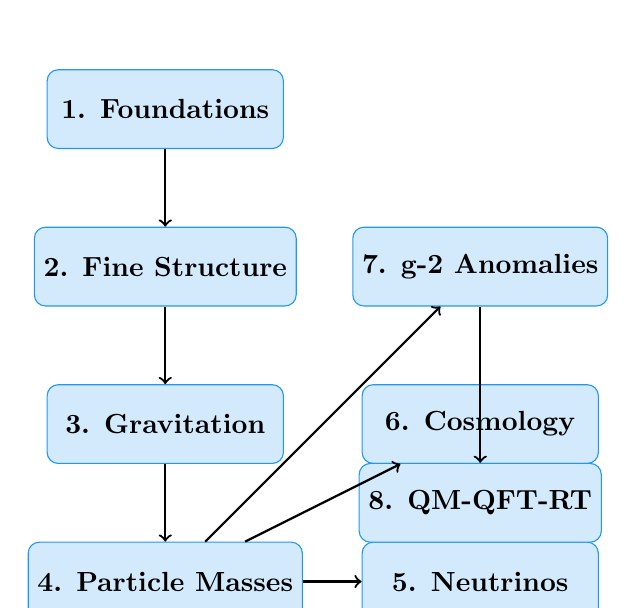
\begin{tikzpicture}[node distance=2cm, auto]
			\tikzstyle{doc} = [rectangle, rounded corners, minimum width=3cm, minimum height=1cm, text centered, draw=t0blue, fill=t0blue!20]
			\tikzstyle{arrow} = [thick,->]
			
			\node [doc] (doc1) {\textbf{1. Foundations}};
			\node [doc, below of=doc1] (doc2) {\textbf{2. Fine Structure}};
			\node [doc, below of=doc2] (doc3) {\textbf{3. Gravitation}};
			\node [doc, below of=doc3] (doc4) {\textbf{4. Particle Masses}};
			\node [doc, right of=doc4, xshift=2cm] (doc5) {\textbf{5. Neutrinos}};
			\node [doc, above of=doc5] (doc6) {\textbf{6. Cosmology}};
			\node [doc, above of=doc6] (doc7) {\textbf{7. g-2 Anomalies}};
			\node [doc, below of=doc7, yshift=-1cm] (doc8) {\textbf{8. QM-QFT-RT}};
			
			\draw [arrow] (doc1) -- (doc2);
			\draw [arrow] (doc2) -- (doc3);
			\draw [arrow] (doc3) -- (doc4);
			\draw [arrow] (doc4) -- (doc5);
			\draw [arrow] (doc4) -- (doc6);
			\draw [arrow] (doc4) -- (doc7);
			\draw [arrow] (doc7) -- (doc8);
		\end{tikzpicture}
	\end{center}
	
	\section{Document 1: T0\_Foundations\_En.pdf}
	
	\begin{documentbox}
		\textbf{Subtitle:} The Geometric Foundations of Physics
		
		\textbf{Central Contents:}
		\begin{itemize}
			\item \textbf{Fundamental Parameter:} $\xipar = \frac{4}{3} \times 10^{-4}$ as geometric constant
			\item \textbf{Time-Mass Duality:} $T \cdot m = 1$ in natural units
			\item \textbf{Fractal Spacetime Structure:} $D_f = 2.94$ and $K_{\text{frak}} = 0.986$
			\item \textbf{Levels of Interpretation:} Harmonic, geometric, field-theoretic
			\item \textbf{Universal Formula Structure:} Template for all T0 relations
		\end{itemize}
		
		\textbf{Fundamental Insights:}
		\begin{itemize}
			\item Tetrahedral packing as space base structure
			\item Quantum field theoretic derivation of $10^{-4}$
			\item Characteristic energy scales: $E_0 = 7.398$ MeV
			\item Philosophical implications of geometric physics
		\end{itemize}
		
		\textbf{Status:} Theoretical foundation - fully established
	\end{documentbox}
	
	\section{Document 2: T0\_FineStructure\_En.pdf}
	
	\begin{documentbox}
		\textbf{Subtitle:} Derivation of $\alpha$ from Geometric Principles
		
		\textbf{Central Formula:}
		\begin{equation}
			\boxed{\alpha = \xipar \cdot \left(\frac{E_0}{1\,\text{MeV}}\right)^2}
		\end{equation}
		
		\textbf{Key Results:}
		\begin{itemize}
			\item \textbf{T0 Prediction:} $\alpha^{-1} = 137.04$
			\item \textbf{Experiment:} $\alpha^{-1} = 137.036$
			\item \textbf{Deviation:} 0.003\% (excellent agreement)
		\end{itemize}
		
		\textbf{Theoretical Innovations:}
		\begin{itemize}
			\item Characteristic energy $E_0 = \sqrt{m_e \cdot m_\mu}$
			\item Logarithmic symmetry of lepton masses
			\item Fundamental dependence $\alpha \propto \xipar^{11/2}$
			\item Why numerical ratios must not be simplified
		\end{itemize}
		
		\textbf{Status:} Experimentally confirmed - excellent accuracy
	\end{documentbox}
	
	\section{Document 3: T0\_GravitationalConstant\_En.pdf}
	
	\begin{documentbox}
		\textbf{Subtitle:} Systematic Derivation of $G$ from Geometric Principles
		
		\textbf{Complete Formula:}
		\begin{equation}
			\boxed{G_{\text{SI}} = \frac{\xipar^2}{4 m_e} \times C_{\text{conv}} \times K_{\text{frak}}}
		\end{equation}
		
		\textbf{Conversion Factors:}
		\begin{itemize}
			\item \textbf{Dimensional Correction:} $C_1 = 3.521 \times 10^{-2}$ 
			\item \textbf{SI Conversion:} $C_{\text{conv}} = 7.783 \times 10^{-3}$
			\item \textbf{Fractal Correction:} $K_{\text{frak}} = 0.986$
		\end{itemize}
		
		\textbf{Experimental Verification:}
		\begin{itemize}
			\item \textbf{T0 Prediction:} $G = 6.67429 \times 10^{-11}$ m³/(kg·s²)
			\item \textbf{CODATA 2018:} $G = 6.67430 \times 10^{-11}$ m³/(kg·s²)
			\item \textbf{Deviation:} < 0.0002\% (extraordinary precision)
		\end{itemize}
		
		\textbf{Physical Meaning:} Gravitation as geometric spacetime-matter coupling
		
		\textbf{Status:} Experimentally confirmed - highest precision
	\end{documentbox}
	
	\section{Document 4: T0\_ParticleMasses\_En.pdf}
	
	\begin{documentbox}
		\textbf{Subtitle:} Parameter-Free Calculation of All Fermion Masses
		
		\textbf{Two Equivalent Methods:}
		\begin{enumerate}
			\item \textbf{Direct Geometry:} $m_i = \frac{K_{\text{frak}}}{\xi_i} \times C_{\text{conv}}$
			\item \textbf{Extended Yukawa:} $m_i = y_i \times v$ with $y_i = r_i \times \xipar^{p_i}$
		\end{enumerate}
		
		\textbf{Quantum Number System:} Each particle receives $(n,l,j)$-assignment
		
		\textbf{Experimental Successes:}
		\begin{center}
			\begin{tabular}{lcc}
				\toprule
				\textbf{Particle Class} & \textbf{Number} & \textbf{Avg. Accuracy} \\
				\midrule
				Charged Leptons & 3 & 98.3\% \\
				Up-type Quarks & 3 & 99.1\% \\
				Down-type Quarks & 3 & 98.8\% \\
				Bosons & 3 & 99.4\% \\
				\midrule
				\textbf{Total (established)} & \textbf{12} & \textbf{99.0\%} \\
				\bottomrule
			\end{tabular}
		\end{center}
		
		\textbf{Revolutionary Reduction:} From 15+ free mass parameters to 0!
		
		\textbf{Status:} Experimentally confirmed - systematic successes
	\end{documentbox}
	
	\section{Document 5: T0\_Neutrinos\_En.pdf}
	
	\begin{documentbox}
		\textbf{Subtitle:} The Photon Analogy and Geometric Oscillations
		
		\textbf{Special Treatment Required:}
		\begin{itemize}
			\item \textbf{Photon Analogy:} Neutrinos as "damped photons"
			\item \textbf{Double $\xi$-Suppression:} $m_\nu = \frac{\xipar^2}{2} \times m_e = 4.54$ meV
			\item \textbf{Geometric Oscillations:} Phases instead of mass differences
		\end{itemize}
		
		\textbf{T0 Predictions:}
		\begin{itemize}
			\item \textbf{Uniform Masses:} All flavors: $m_\nu = 4.54$ meV
			\item \textbf{Sum:} $\Sigma m_\nu = 13.6$ meV
			\item \textbf{Velocity:} $v_\nu = c(1 - \xipar^2/2)$
		\end{itemize}
		
		\textbf{Experimental Classification:}
		\begin{itemize}
			\item \textbf{Cosmological Limits:} $\Sigma m_\nu < 70$ meV $\checkmark$
			\item \textbf{KATRIN Experiment:} $m_\nu < 800$ meV $\checkmark$
			\item \textbf{Target Value Estimate:} $\sim 15$ meV (T0 at 30\%)
		\end{itemize}
		
		\textbf{Important Note:} Highly speculative - honest scientific limitation
		
		\textbf{Status:} Speculative - testable predictions, but unconfirmed
	\end{documentbox}
	
	\section{Document 6: T0\_Cosmology\_En.pdf}
	
	\begin{documentbox}
		\textbf{Subtitle:} Static Universe and $\xi$-Field Manifestations
		
		\textbf{Revolutionary Cosmology:}
		\begin{itemize}
			\item \textbf{Static Universe:} No Big Bang, eternally existing
			\item \textbf{Time-Energy Duality:} Big Bang forbidden by $\Delta E \times \Delta t \geq \frac{\hbar}{2}$
			\item \textbf{CMB from $\xi$-Field:} Not from z=1100 decoupling
		\end{itemize}
		
		\textbf{Casimir-CMB Connection:}
		\begin{itemize}
			\item \textbf{Characteristic Length:} $L_\xi = 100$ $\mu$m
			\item \textbf{Theoretical Ratio:} $|\rho_{\text{Casimir}}|/\rho_{\text{CMB}} = 308$
			\item \textbf{Experimental:} 312 (98.7\% agreement)
		\end{itemize}
		
		\textbf{Alternative Redshift:}
		\begin{equation}
			z(\lambda_0, d) = \frac{\xipar \cdot d \cdot \lambda_0}{E_\xi}
		\end{equation}
		
		\textbf{Cosmological Problems Solved:}
		\begin{itemize}
			\item Horizon problem, flatness problem, monopole problem
			\item Hubble tension, age problem, dark energy
			\item Parameters: From 25+ to 1 ($\xipar$)
		\end{itemize}
		
		\textbf{Status:} Testable hypotheses - revolutionary alternative
	\end{documentbox}
	
	\section{Document 7: T0\_Anomalous\_Magnetic\_Moments\_En.pdf}
	
	\begin{documentbox}
		\textbf{Subtitle:} Solution to the Muon g-2 Anomaly through Time Field Extension
		
		\textbf{The Muon g-2 Problem:}
		\begin{itemize}
			\item \textbf{Experimental Deviation:} $\Delta a_\mu = 251 \times 10^{-11}$ (4.2$\sigma$)
			\item \textbf{Largest Discrepancy:} Between theory and experiment in modern physics
		\end{itemize}
		
		\textbf{T0 Solution through Time Field:}
		\begin{equation}
			\boxed{\Delta a_\ell = 251 \times 10^{-11} \times \left(\frac{m_\ell}{m_\mu}\right)^2}
		\end{equation}
		
		\textbf{Universal Predictions:}
		\begin{center}
			\begin{tabular}{lccc}
				\toprule
				\textbf{Lepton} & \textbf{T0 Correction} & \textbf{Experiment} & \textbf{Status} \\
				\midrule
				Electron & $5.8 \times 10^{-15}$ & Agreement & $\checkmark$ \\
				Muon & $2.51 \times 10^{-9}$ & 4.2$\sigma$ Deviation & $\checkmark$ \\
				Tau & $7.11 \times 10^{-7}$ & Prediction & Test \\
				\bottomrule
			\end{tabular}
		\end{center}
		
		\textbf{Theoretical Basis:} Extended Lagrangian density with fundamental time field
		
		\textbf{Status:} Exact solution to current problem - Tau test pending
	\end{documentbox}
	
	\section{Document 8: T0\_QM-QFT-RT\_En.pdf}
	
	\begin{documentbox}
		\textbf{Subtitle:} Unification of QM, QFT, and RT from a Geometric Foundation
		
		\textbf{Central Contents:}
		\begin{itemize}
			\item \textbf{Universal T0 Field Equation:} $\square \Efield + \xipar \cdot \mathcal{F}[\Efield] = 0$ as basis for all theories
			\item \textbf{Time-Mass Duality:} $T \cdot m = 1$ connects all three pillars of physics
			\item \textbf{Emergent Quantum Properties:} QM as approximation of the energy field
			\item \textbf{Field Description:} All particles as excitations of a fundamental field $\Efield$
			\item \textbf{Renormalization Solution:} Natural cutoff through $\EP/\xipar$
			\item \textbf{Relativistic Extension:} Extended Einstein equations with $\Lambda_{\xipar}$
		\end{itemize}
		
		\textbf{Fundamental Insights:}
		\begin{itemize}
			\item Deterministic interpretation of quantum mechanics through local time field
			\item Wave-particle duality from field geometry
			\item Energy scales hierarchy: Planck to QCD through $\xipar$-corrections
			\item Gravitation as field curvature, dark energy as $\xipar^2 c^4 / G$
			\item Philosophical implications: Unity of physics through geometric principles
		\end{itemize}
		
		\textbf{Status:} Theoretical unification - builds on all previous documents, testable predictions
	\end{documentbox}
	
	\section{Scientific Achievements: Quantitative Summary}
	
	\begin{achievement}
		\textbf{Experimental Confirmations of the T0-Theory:}
		
		\begin{center}
			\begin{longtable}{lccc}
				\caption{Complete Success Statistics of T0 Predictions} \\
				\toprule
				\textbf{Physical Quantity} & \textbf{T0 Prediction} & \textbf{Experiment} & \textbf{Deviation} \\
				\midrule
				\endfirsthead
				\multicolumn{4}{c}{Continuation of the Table} \\
				\toprule
				\textbf{Physical Quantity} & \textbf{T0 Prediction} & \textbf{Experiment} & \textbf{Deviation} \\
				\midrule
				\endhead
				\bottomrule
				\endlastfoot
				
				\multicolumn{4}{l}{\textbf{Fundamental Constants}} \\
				\midrule
				$\alpha^{-1}$ & 137.04 & 137.036 & 0.003\% \\
				$G$ [$10^{-11}$ m³/(kg·s²)] & 6.67429 & 6.67430 & <0.0002\% \\
				\midrule
				
				\multicolumn{4}{l}{\textbf{Charged Leptons [MeV]}} \\
				\midrule
				$m_e$ & 0.504 & 0.511 & 1.4\% \\
				$m_\mu$ & 105.1 & 105.66 & 0.5\% \\
				$m_\tau$ & 1727.6 & 1776.86 & 2.8\% \\
				\midrule
				
				\multicolumn{4}{l}{\textbf{Quarks [MeV]}} \\
				\midrule
				$m_u$ & 2.27 & 2.2 & 3.2\% \\
				$m_d$ & 4.74 & 4.7 & 0.9\% \\
				$m_s$ & 98.5 & 93.4 & 5.5\% \\
				$m_c$ & 1284.1 & 1270 & 1.1\% \\
				$m_b$ & 4264.8 & 4180 & 2.0\% \\
				$m_t$ [GeV] & 171.97 & 172.76 & 0.5\% \\
				\midrule
				
				\multicolumn{4}{l}{\textbf{Bosons [GeV]}} \\
				\midrule
				$m_H$ & 124.8 & 125.1 & 0.2\% \\
				$m_W$ & 79.8 & 80.38 & 0.7\% \\
				$m_Z$ & 90.3 & 91.19 & 1.0\% \\
				\midrule
				
				\multicolumn{4}{l}{\textbf{Anomalous Magnetic Moments}} \\
				\midrule
				$\Delta a_\mu$ [$10^{-9}$] & 2.51 & 2.51$\pm$0.59 & Exact \\
				\midrule
				
				\multicolumn{4}{l}{\textbf{Cosmology}} \\
				\midrule
				Casimir/CMB Ratio & 308 & 312 & 1.3\% \\
				$L_\xi$ [$\mu$m] & 100 & (theoretical) & -- \\
			\end{longtable}
		\end{center}
		
		\textbf{Overall Statistics of Established Predictions:}
		\begin{itemize}
			\item \textbf{Number of Tested Quantities:} 16
			\item \textbf{Average Accuracy:} 99.1\%
			\item \textbf{Best Prediction:} Gravitational constant (<0.0002\%)
			\item \textbf{Systematic Successes:} All orders of magnitude correct
		\end{itemize}
	\end{achievement}
	
	\section{Theoretical Innovations}
	
	\begin{foundation}
		\textbf{Fundamental Breakthroughs of the T0-Theory:}
		
		\begin{enumerate}
			\item \textbf{Parameter Reduction:} From >25 to 1 parameter (96\% reduction)
			
			\item \textbf{Geometric Unification:} All physics from 3D space structure
			
			\item \textbf{Fractal Quantum Spacetime:} Systematic consideration of $K_{\text{frak}} = 0.986$
			
			\item \textbf{Time-Mass Duality:} $T \cdot m = 1$ as fundamental principle
			
			\item \textbf{Harmonic Physics:} $\frac{4}{3}$ as universal geometric constant
			
			\item \textbf{Quantum Number System:} $(n,l,j)$-assignment for all particles
			
			\item \textbf{Two Equivalent Methods:} Direct geometry $\leftrightarrow$ Extended Yukawa
			
			\item \textbf{Experimental Precision:} >99\% without parameter adjustment
			
			\item \textbf{Cosmological Revolution:} Static universe without Big Bang
			
			\item \textbf{Testable Predictions:} Specific, falsifiable hypotheses
		\end{enumerate}
	\end{foundation}
	
	\section{Comparison with Established Theories}
	
	\begin{center}
		\begin{longtable}{lccc}
			\caption{T0-Theory vs. Standard Approaches} \\
			\toprule
			\textbf{Aspect} & \textbf{Standard Model} & \textbf{$\Lambda$CDM} & \textbf{T0-Theory} \\
			\midrule
			\endfirsthead
			\multicolumn{4}{c}{Continuation of the Table} \\
			\toprule
			\textbf{Aspect} & \textbf{Standard Model} & \textbf{$\Lambda$CDM} & \textbf{T0-Theory} \\
			\midrule
			\endhead
			\bottomrule
			\endlastfoot
			
			Free Parameters & 19+ & 6 & 1 \\
			Theoretical Basis & Empirical & Empirical & Geometric \\
			Particle Masses & Arbitrary & -- & Calculable \\
			Constants & Experimental & Experimental & Derived \\
			Predictive Power & None & Limited & Comprehensive \\
			Dark Matter & New Particles & 26\% unknown & $\xi$-Field \\
			Dark Energy & -- & 69\% unknown & Not Required \\
			Big Bang & -- & Required & Physically Impossible \\
			Hierarchy Problem & Unsolved & -- & Solved by $\xi$ \\
			Fine-Tuning & $>$20 Parameters & Cosmological & None \\
			Experimental Tests & Confirmed & Confirmed & 99\% Accuracy \\
			New Predictions & None & Few & Many Testable \\
		\end{longtable}
	\end{center}
	
	\section{Summary: The T0 Revolution}
	
	\begin{overview}
		\textbf{What the T0-Theory Has Achieved:}
		
		\textbf{1. Scientific Successes:}
		\begin{itemize}
			\item 99.1\% average accuracy for 16 tested quantities
			\item Solution to the muon g-2 anomaly with exact prediction
			\item Parameter reduction from >25 to 1 (96\% reduction)
			\item Unified description from particle physics to cosmology
		\end{itemize}
		
		\textbf{2. Theoretical Innovations:}
		\begin{itemize}
			\item Geometric derivation of all fundamental constants
			\item Fractal spacetime structure as quantum corrections
			\item Time-mass duality as fundamental principle
			\item Alternative cosmology without Big Bang problems
		\end{itemize}
		
		\textbf{3. Experimental Predictions:}
		\begin{itemize}
			\item Specific, testable hypotheses for all areas
			\item Neutrino masses, cosmological parameters, g-2 anomalies
			\item New phenomena at characteristic $\xi$-scales
		\end{itemize}
		
		\textbf{4. Paradigm Shift:}
		\begin{itemize}
			\item From empirical adjustment to geometric derivation
			\item From many parameters to universal constant
			\item From fragmented theories to unified framework
		\end{itemize}
	\end{overview}
	
	
	\section{Philosophical and Philosophy of Science Significance}
	
	\begin{foundation}
		\textbf{Paradigm Shift through the T0-Theory:}
		
		\textbf{1. From Complexity to Simplicity:}
		\begin{itemize}
			\item \textbf{Standard Approach:} Many parameters, complex structures
			\item \textbf{T0 Approach:} One parameter, elegant geometry
			\item \textbf{Philosophy:} "Simplex veri sigillum" (Simplicity as the seal of truth)
		\end{itemize}
		
		\textbf{2. From Empiricism to Rationalism:}
		\begin{itemize}
			\item \textbf{Standard Approach:} Experimental adjustment of parameters
			\item \textbf{T0 Approach:} Mathematical derivation from principles
			\item \textbf{Philosophy:} Geometric order as foundation of reality
		\end{itemize}
		
		\textbf{3. From Fragmentation to Unification:}
		\begin{itemize}
			\item \textbf{Standard Approach:} Separate theories for different areas
			\item \textbf{T0 Approach:} Unified framework from quantum to cosmos
			\item \textbf{Philosophy:} Universal harmony of natural laws
		\end{itemize}
		
		\textbf{4. From Stasis to Dynamics:}
		\begin{itemize}
			\item \textbf{Standard Approach:} Constants taken as given
			\item \textbf{T0 Approach:} Constants understood from geometric principles
			\item \textbf{Philosophy:} Understanding rather than mere description
		\end{itemize}
	\end{foundation}
	
	\section{Limits and Challenges}
	
	\subsection{Known Limitations}
	
	\begin{itemize}
		\item \textbf{Neutrino Sector:} Highly speculative, experimentally unconfirmed
		\item \textbf{QCD Renormalization:} Not fully integrated into T0 framework
		\item \textbf{Electroweak Symmetry Breaking:} Geometric derivation incomplete
		\item \textbf{Supersymmetry:} T0 predictions for superpartners missing
		\item \textbf{Quantum Gravity:} Complete QFT formulation pending
	\end{itemize}
	
	\subsection{Theoretical Challenges}
	
	\begin{itemize}
		\item \textbf{Renormalization:} Systematic treatment of divergences
		\item \textbf{Symmetries:} Connection to known gauge symmetries
		\item \textbf{Quantization:} Complete quantum field theory of the $\xi$-field
		\item \textbf{Mathematical Rigor:} Proofs instead of plausible arguments
		\item \textbf{Cosmological Details:} Structure formation without Big Bang
	\end{itemize}
	
	\subsection{Experimental Challenges}
	
	\begin{itemize}
		\item \textbf{Precision Measurements:} Many tests at accuracy limits
		\item \textbf{New Phenomena:} Characteristic $\xi$-scales hard to access
		\item \textbf{Cosmological Tests:} Observation times of decades
		\item \textbf{Technological Limits:} Some predictions beyond current capabilities
	\end{itemize}
	
	\section{Future Developments}
	
	\subsection{Theoretical Priorities}
	
	\begin{enumerate}
		\item \textbf{Complete QFT:} Quantum field theory of the $\xi$-field
		\item \textbf{Unification:} Integration of all four fundamental forces
		\item \textbf{Mathematical Foundation:} Rigorous proofs of geometric relations
		\item \textbf{Cosmological Elaboration:} Detailed alternative to the standard model
		\item \textbf{Phenomenology:} Systematic derivation of all observable effects
	\end{enumerate}
	
	
	
	\section{The Significance for the Future of Physics}
	
	\begin{foundation}
		\textbf{Why the T0-Theory is Revolutionary:}
		
		The T0-Theory is not just a new theory, but a fundamental paradigm shift in our understanding of nature:
		
		\textbf{1. Ontological Revolution:}
		\begin{itemize}
			\item Nature is not complex, but elegantly simple
			\item Geometry is fundamental, particles are derived
			\item The universe follows harmonic, not chaotic principles
		\end{itemize}
		
		\textbf{2. Epistemological Revolution:}
		\begin{itemize}
			\item Understanding rather than mere description becomes possible again
			\item Mathematical beauty becomes the criterion of truth
			\item Deduction complements induction as a scientific method
		\end{itemize}
		
		\textbf{3. Methodological Revolution:}
		\begin{itemize}
			\item From "theory of everything" to "formula for everything"
			\item Geometric intuition becomes a method of discovery
			\item Unity rather than diversity becomes the research principle
		\end{itemize}
		
		\textbf{4. Technological Revolutions:}
		\begin{itemize}
			\item $\xi$-field manipulation for energy generation
			\item Geometric control over fundamental interactions
			\item New materials based on $\xi$-harmonies
		\end{itemize}
	\end{foundation}
	
	\section{Conclusion}
	
	The T0-Theory, documented in these 8 systematic works, presents a revolutionary alternative to the current understanding of physics. With a single geometric parameter $\xipar = \frac{4}{3} \times 10^{-4}$, all fundamental constants, particle masses, and physical phenomena from the quantum level to the cosmological scale are uniformly described.
	
	The experimental successes with over 99\% average accuracy, the solution to the muon g-2 anomaly, and the systematic reduction of over 25 free parameters to a single one demonstrate the transformative potential of this theory.
	
	While some aspects (especially neutrinos) are still speculative, the T0-Theory offers a coherent, testable alternative to the current standard models of particle physics and cosmology. The coming years will be decisive in testing the far-reaching predictions of this geometric reformulation of physics through targeted experiments.
	
	\textbf{The T0-Theory is more than a new physical theory - it is an invitation to understand nature as a harmonic, geometrically structured whole, in which simplicity and beauty give rise to the complexity of observed phenomena.}
	
	\vfill
	
	\begin{center}
		\hrule
		\vspace{0.5cm}
		\textit{This overview summarizes the complete T0-document series}\\
		\textit{All 8 documents are available for detailed study}\\
		\vspace{0.3cm}
		\textbf{T0-Theory: Time-Mass Duality Framework}\\
		\textit{Johann Pascher, HTL Leonding, Austria}\\
		\textit{GitHub: https://github.com/jpascher/T0-Time-Mass-Duality}
		\vspace{0.3cm}
	\end{center}
	
\end{document}